\documentclass[14 pt]{extarticle}

	\usepackage[frenchb]{babel}
	\usepackage[utf8]{inputenc}  
	\usepackage[T1]{fontenc}
	\usepackage{amssymb}
	\usepackage[mathscr]{euscript}
	\usepackage{stmaryrd}
	\usepackage{amsmath}
	\usepackage{tikz}
	\usepackage[all,cmtip]{xy}
	\usepackage{amsthm}
	\usepackage{varioref}
	\usepackage{geometry}
	\geometry{a4paper}
	\usepackage{lmodern}
	\usepackage{hyperref}
	\usepackage{array}
	 \usepackage{fancyhdr}
	 \usepackage{float}
\renewcommand{\theenumi}{\alph{enumi})}
	\pagestyle{fancy}
	\theoremstyle{plain}
	\fancyfoot[C]{} 
	\fancyhead[L]{Contrôle}
	\fancyhead[R]{9 octobre 2024}\geometry{
 a4paper,
 total={190mm,257mm},
 left=10mm,
 top=20mm,
 }
	
	
	\title{Contrôle Chapitre 2}
	\date{}
	\begin{document}

\begin{center}{\Large Interrogation Chapitre 2}\\ 
 \end{center}
 Nom : \\
 Prénom : \\
 \subsection*{Exercice 1 (3 points)}
 Calculez, \emph{en détaillant les étapes} : 
 \begin{enumerate}
 \item $2 + 3 \times 4$
 \item $(17 -1 + 4) \div 2 +2 $
 \item $ (10 + 5)\div 3 \times 5$
 \end{enumerate}
 \subsection*{Exercice 2 (2 points)}
 
 Rappelez la définition de la médiatrice d'un segment $[AB]$. 
 
 \subsection*{Exercice 3 (12 points)}
 
 Tracez les symétriques des figures suivantes par rapport à la droite $(d)$.
 
 \begin{figure}[H]
 \center
 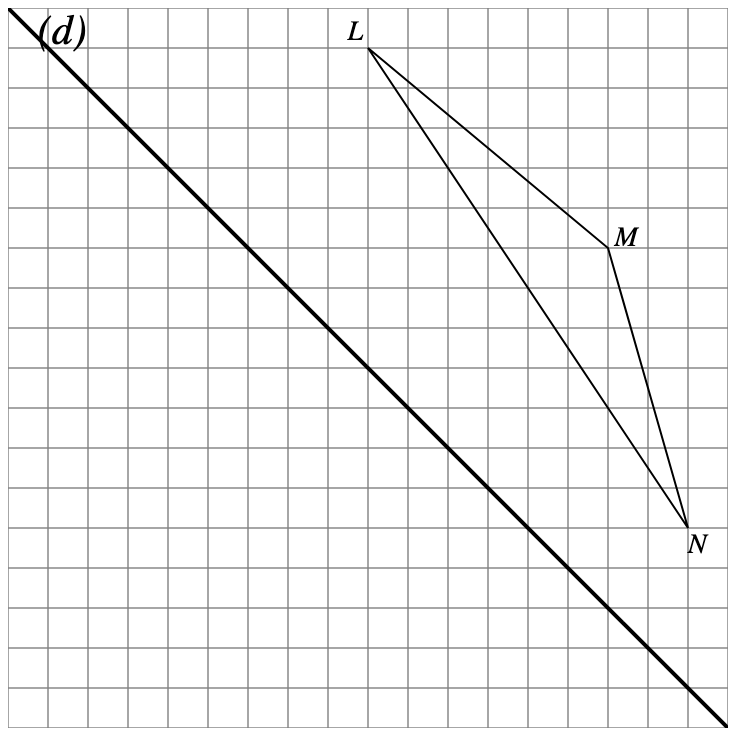
\includegraphics[scale=.65]{Fig1}
 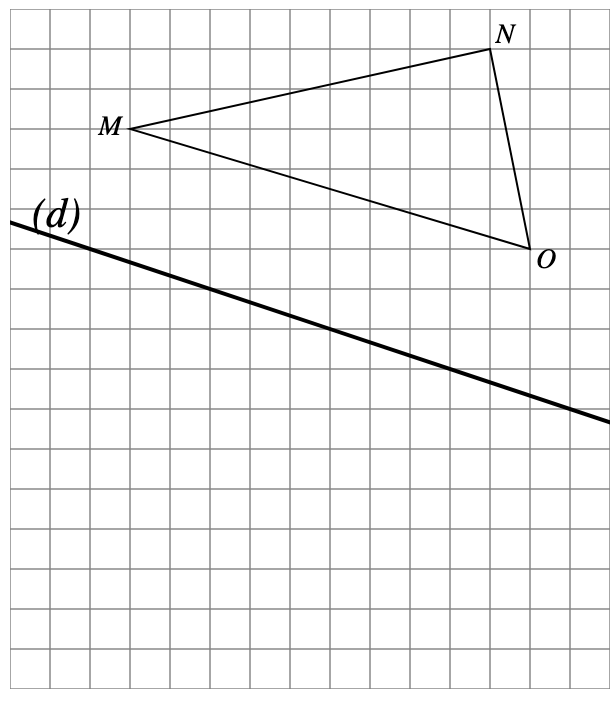
\includegraphics[scale=.65]{Fig2}
 \end{figure}
 \newpage
  \begin{figure}[H]
 \center
 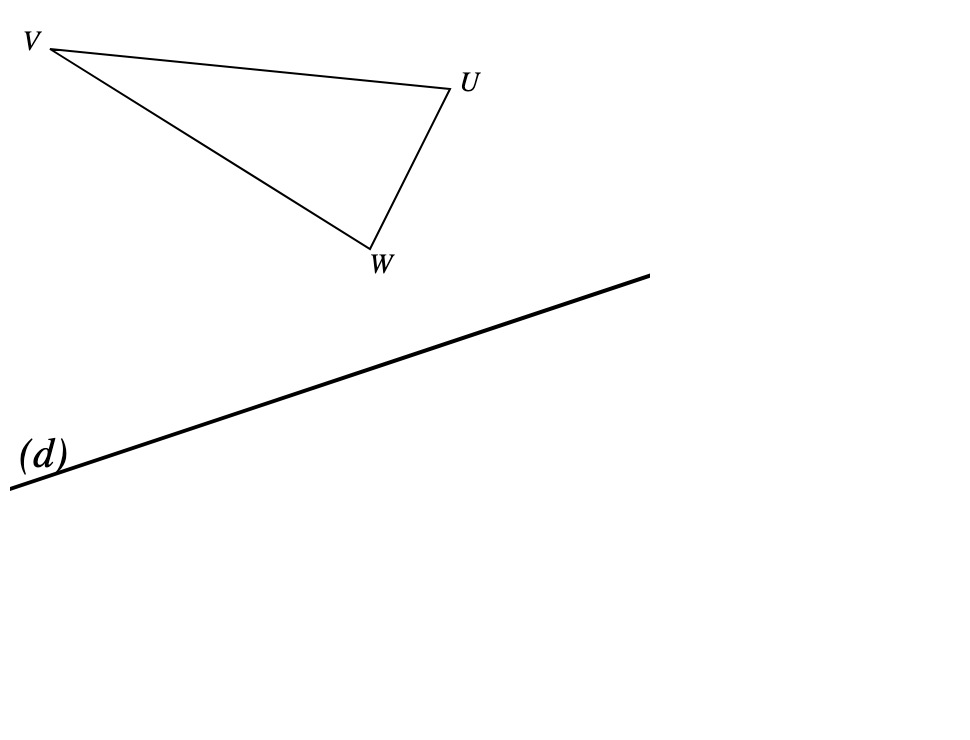
\includegraphics[scale=.6]{Fig4}
 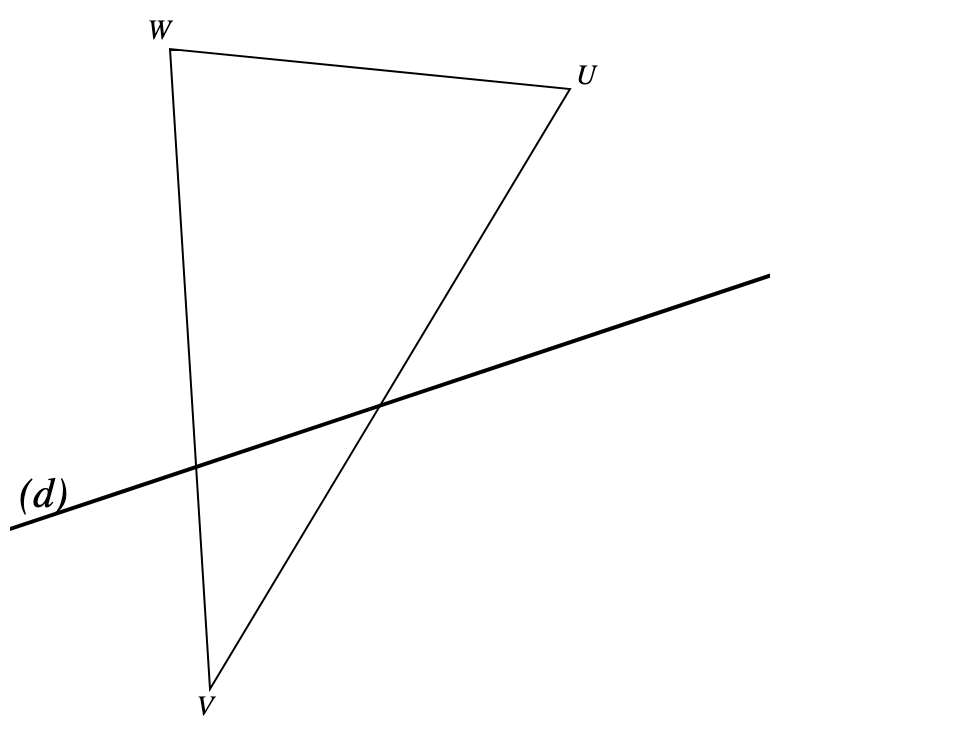
\includegraphics[scale=.5]{Fig3}
 \end{figure}
 
\subsection*{Exercice 4 (3 points)} 

Sur les figures suivantes, représentez les axes de symétrie éventuels, et dites leur nombre.  

\begin{figure}[H]
\center 

\includegraphics[scale=.06]{Niger.png}\ \ \ \ \ 

\includegraphics[scale=.06]{Suisse.png}\ \ \ \ \ 

\includegraphics[scale=.06]{Honduras.png}
\end{figure}
 

\newpage

\begin{center}{\Large Interrogation Chapitre 2}\\ 
 \end{center}
 Nom : \\
 Prénom : \\
 \subsection*{Exercice 1 (3 points)}
 Calculez, \emph{en détaillant les étapes} : 
 \begin{enumerate}
 \item $2 + 5 \times 4$
 \item $(17 -2 + 3) \div 2 +2 $
 \item $ (10 + 5)\div 3 \times 5$
 \end{enumerate}
 \subsection*{Exercice 2 (2 points)}
 
 Rappelez la définition de la médiatrice d'un segment $[CD]$. 
 
 \subsection*{Exercice 3 (12 points)}
 
 Tracez les symétriques des figures suivantes par rapport à la droite $(d)$.
 
 \begin{figure}[H]
 \center
 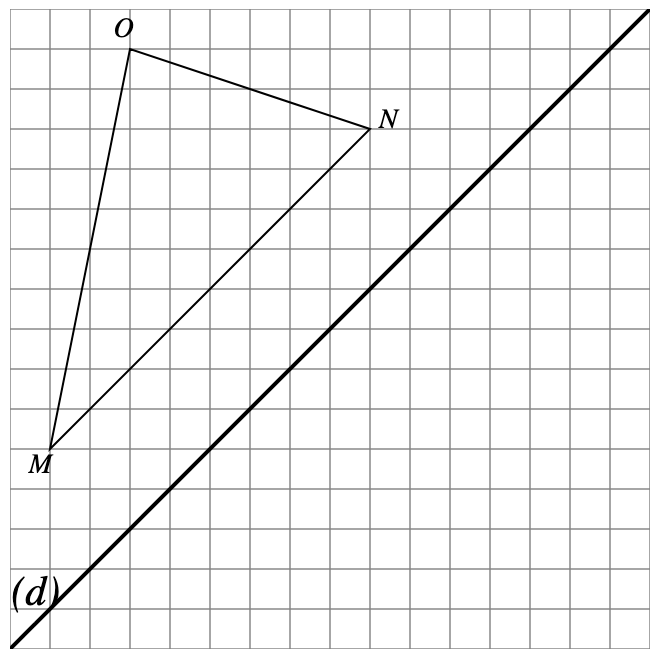
\includegraphics[scale=.65]{Fig1b}
 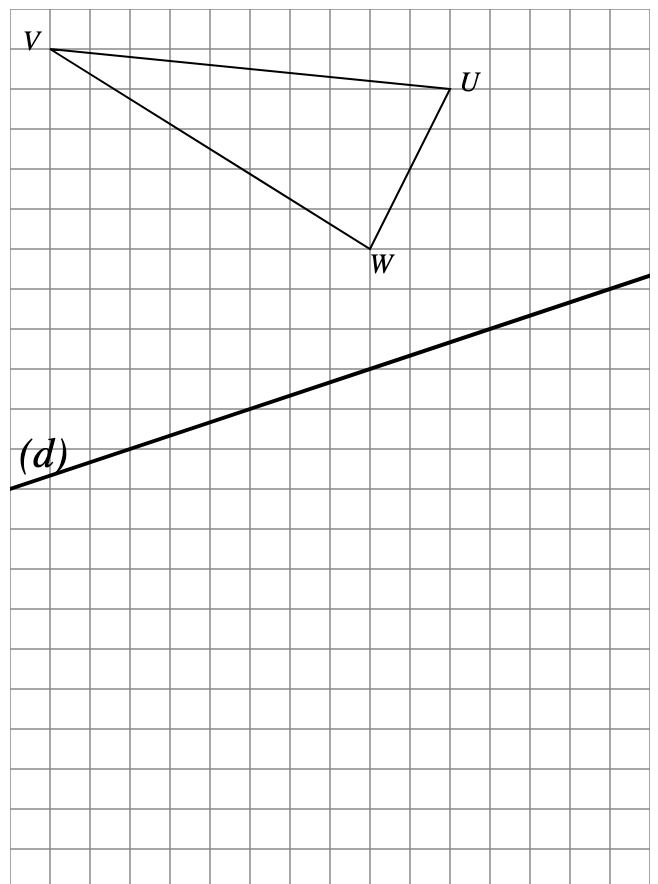
\includegraphics[scale=.65]{Fig2b}
 \end{figure}
 \newpage
  \begin{figure}[H]
 \center
 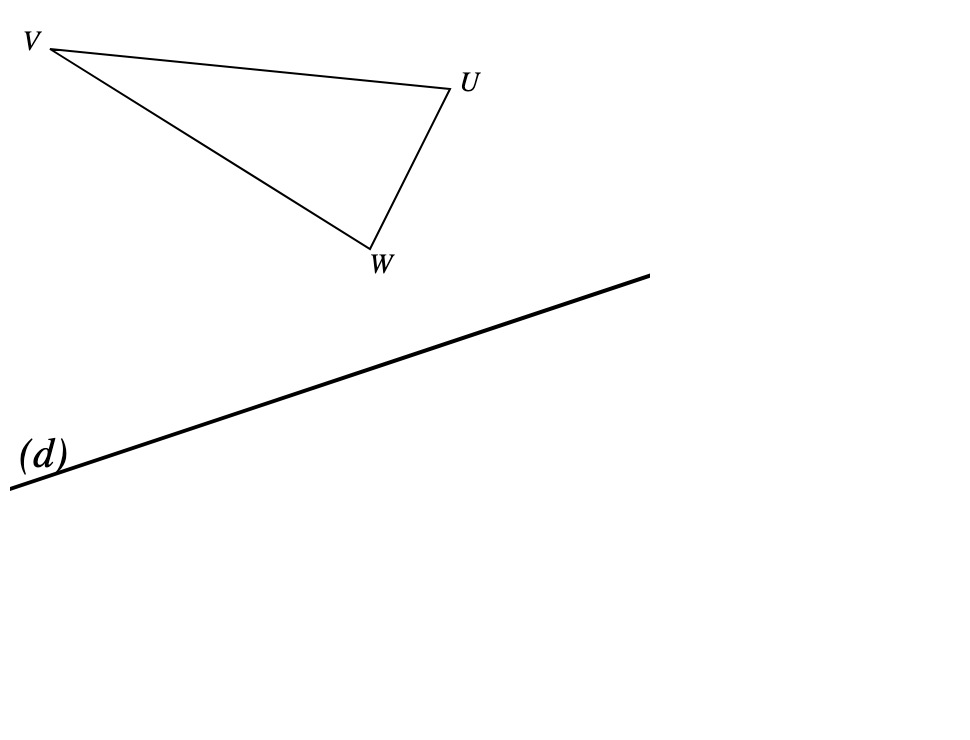
\includegraphics[scale=.6]{Fig4}\\
 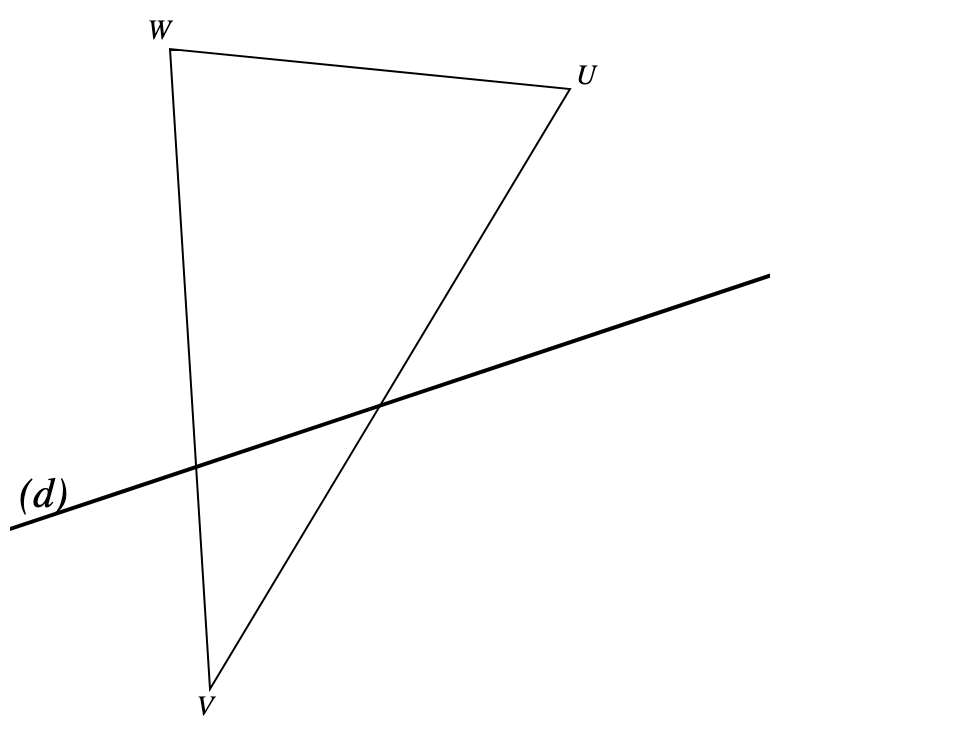
\includegraphics[scale=.6]{Fig3}
 \end{figure}
 
\subsection*{Exercice 4 (3 points)} 

Sur les figures suivantes, représentez les axes de symétrie éventuels, et dites leur nombre.  

\begin{figure}[H]
\center 

\includegraphics[scale=.06]{Vietnam.png}\ \ \ \ \ 

\includegraphics[scale=.06]{Suisse.png}\ \ \ \ \ 

\includegraphics[scale=.06]{Honduras.png}
\end{figure}







 	\end{document}
